\documentclass[11pt,a4paper]{article}
\usepackage{vntex}
\usepackage{hyperref}
\usepackage{enumerate}
\usepackage{graphicx}
\usepackage[left=3cm, right=2cm, top=3cm, bottom=3cm]{geometry}
\usepackage[utf8]{inputenc}
\usepackage{fancyhdr}
\usepackage{lastpage}
\usepackage{indentfirst}
\usepackage{listings}
\usepackage{color}
 
\definecolor{codegreen}{rgb}{0,0.6,0}
\definecolor{codegray}{rgb}{0.5,0.5,0.5}
\definecolor{codepurple}{rgb}{0.58,0,0.82}
\definecolor{backcolour}{rgb}{0.95,0.95,0.92}

\lstdefinestyle{mystyle}{
    backgroundcolor=\color{backcolour},   
    commentstyle=\color{codegreen},
    keywordstyle=\color{magenta},
    numberstyle=\tiny\color{codegray},
    stringstyle=\color{codepurple},
    basicstyle=\footnotesize,
    breakatwhitespace=false,         
    breaklines=true,                 
    captionpos=b,                    
    keepspaces=true,                 
    numbers=left,                    
    numbersep=5pt,                  
    showspaces=false,                
    showstringspaces=false,
    showtabs=false,
    tabsize=2
}

\lstset{style=mystyle}


\title{Luận văn tốt nghiệp}
\author{Nguyễn Hữu Phương}
\date{March 2020}

\pagestyle{fancy}
\fancyhead{}
\fancyhead[L]{
 \begin{tabular}{rl}
    \begin{picture}(25,15)(0,0)
    \put(0,-8){
\includegraphics[width=8mm, height=8mm]{fig/hcmut.jpg}}
    %\put(0,-8){\epsfig{width=10mm,figure=hcmut.eps}}
   \end{picture}&
	%
\includegraphics[width=8mm, height=8mm]{hcmut.jpg} & %
	\begin{tabular}{l}
		\textbf{\bf \ttfamily Trường Đại Học Bách Khoa Tp.Hồ Chí Minh}\\
		\textbf{\bf \ttfamily Khoa Khoa Học và Kỹ Thuật Máy Tính}
	\end{tabular} 	
 \end{tabular}
}
\fancyhead[R]{
	\begin{tabular}{l}
		\tiny \bf \\
		\tiny \bf 
	\end{tabular}  }
\fancyfoot{} % clear all footer fields
\fancyfoot[L]{\scriptsize \ttfamily Luận văn tốt nghiệp }
\fancyfoot[R]{\scriptsize \ttfamily Trang {\thepage}/\pageref{LastPage}}
\renewcommand{\headrulewidth}{0.3pt}
\renewcommand{\footrulewidth}{0.3pt}

\begin{document}

%% --------- TITLE PAGE ---------
\begin{titlepage}
\begin{center}
    ĐẠI HỌC QUỐC GIA THÀNH PHỐ HỒ CHÍ MINH\\
    TRƯỜNG ĐẠI HỌC BÁCH KHOA\\
    KHOA KHOA HỌC VÀ KỲ THUẬT MÁY TÍNH
\end{center}

\vspace{1cm}

\begin{figure}[h!]
    \centering
    
\includegraphics[scale = 0.2]{fig/hcmut.jpg}
\end{figure}

\vspace{1cm}

\begin{center}
\begin{tabular}{c}
    \multicolumn{1}{l}{\textbf{{\Large LUẬN VĂN TỐT NGHIỆP}}}\\
    ~~\\
    \hline
    \\
    \multicolumn{1}{l}{\textbf{{\Large KỸ THUẬT BẢO VỆ THÔNG TIN RIÊNG TƯ}}}\\
    \\

    \textbf{{\Huge TRONG DỮ LIỆU MỞ}}\\
	\\
    \hline
\end{tabular}
\end{center}

\vspace{3cm}

\begin{table}[h]
\begin{tabular}{rrl}
\hspace{5 cm} & GVHD: &TS. TRƯƠNG TUẤN ANH\\
& GVPB: & \\
& NHÓM SV: & NGUYỄN HỮU PHƯƠNG - 1413022\\
&   & TRẦN LÊ MINH - 1412319\\
&   & NGUYỄN TRUNG TÀI - 1512891 
\end{tabular}
\end{table}

\vspace{2cm}

\begin{center}
{\footnotesize HỒ CHÍ MINH, THÁNG 3/2020}
\end{center}
\end{titlepage}


%% --------- LỜI CAM ĐOAN ---------
\newpage
\section{LỜI CAM ĐOAN:}
Nhóm xin cam đoan đây là công trình nghiên cứu của chúng em và được sự hướng dẫn khoa học của TS. Trương Tuấn Anh. Các nội dung, kết quả thu được trong đề tài này là trung thực, và chưa được công bố trong bất cứ dưới hình thức nào trước đây. Những số liệu phục vụ cho việc phân tích, nhận xét, đánh giá được tôi thu thập từ các nguồn khác nhau có ghi rõ trong tài liệu tham khảo. Ngoài ra, trong tài liệu còn sử dụng một số hình ảnh, nhận xét, đánh giá cũng như số liệu của các tác giả, cơ quan tổ chức khác đều có trích dẫn và chú thích nguồn gốc. Nếu có phát hiện bất cứ gian lận nào, nhóm xin chịu hoàn toàn trách nhiệm về mặt nội dung của luận văn tốt nghiệp của nhóm. Trường Đại học Bách Khoa – Đại Học Quốc Gia Thành Phố Hồ Chí Minh không liên quan đến những vi phạm tác quyền, bản quyền do nhóm gây ra trong quá trình thực hiện (nếu có).
\\

\hspace*{\fill} TP. HỒ CHÍ MINH, ngày 15/03/2020.


%% --------- LỜI CẢM ƠN ---------
\newpage
\section{LỜI CẢM ƠN:}
Em cảm thấy thật may mắn và tự hào khi được học tập, làm việc tại trường Đại học Bách Khoa - Đại học Quốc gia TP.HCM, nơi chúng em được sự chỉ bảo của các thầy cô giáo tận tâm với các thế hệ sinh viên giỏi chuyên môn, đội ngũ kỹ sư chất lượng cao, phục vụ cho việc phát triển đất nước. Bên cạnh đó cũng là sự gắn bó, quan tâm của bạn bè tại trường đã giúp chúng em có một quãng thời gian làm sinh viên thật sự đáng nhớ và đáng trân trọng trong suốt cuộc đời.\\[0.2cm]
Với lòng biết ơn sâu sắc nhất, chúng em xin gửi lời cảm ơn tới thầy Trương Tuấn Anh. Thầy đã tạo điều kiện và cơ hội để tôi được tham gia vào đề tài \textbf{"Kỹ thuật bảo vệ thông tin riêng tư trong dữ liệu mở"}. Trong quá trình tìm hiểu, thầy có vai trò rất quan trọng để nhóm hiểu về đề tài . Qua đó, tôi đã có thể thực hiện tốt nhất đề tài trong khả năng của mình.\\[0.2cm]
Ngoài ra, tôi cũng xin gửi lời cảm ơn chân thành tới các thầy, cô của trường Đại học Bách Khoa - Đại học Quốc gia TP.HCM nói chung cũng như các thầy cô trong Khoa Khoa học và Kỹ thuật Máy Tính nói riêng, đã cung cấp các kiến thức nền tảng để tôi áp dụng vào đề tài luận văn tốt nghiệp này.\\[0.2cm]
Trong quá trình thực hiện đề tài, không tránh khỏi những thiếu sót, vậy nên nhóm rất mong nhận được các ý kiến đóng góp quý báu từ các quý thầy, cô và các bạn sinh viên.\\[0.2cm]
\hspace*{\fill} Xin chân thành cảm ơn!


%% --------- MỤC LỤC ---------
\newpage
\tableofcontents


%% --------- DANH SÁCH TỪ THUẬT NGỮ ---------
\newpage
\section{DANH SÁCH TỪ THUẬT NGỮ}
\begin{tabular}{|l|c|r|}
    \hline
    TỪ VIẾT TẮT & NỘI DUNG \\
    \hline
    Big Data & Dữ liệu lớn \\
    Cluster & Cụm máy tính \\
    Distributed System & Hệ thống tính toán phân tán \\
    Open-source & Mã nguồn mở \\
    Script & Đoạn mã \\
    Machine Learning & Học máy \\
    Port & Cổng \\
    
    
    \hline
\end{tabular}


%% --------- TỔNG QUAN --------
\newpage
\section{TỔNG QUAN}
\subsection{Giới thiệu đề tài}
Hiện nay, vào thời đại công nghiệp 4.0, việc thu thập, khai thác từ dữ liệu mang lại lợi ích không hề nhỏ. Kèm theo đó, công việc xây dựng nên các hệ thống thu thập, phân tích dữ liệu cũng có nhu cầu rất cao, tuy nhiên lại gặp khó khăn khi yêu cầu cho việc xử lý, phân tích Big Data cần các hệ thống máy tính đặc biệt, chuyên dụng, có sức mạnh kèm theo đó là chi phí xây dựng rất lớn. Nhưng việc cài đặt, tinh chỉnh cấu hình các hệ thống như vậy không hoàn toàn quen thuộc với người sử dụng hệ thống đó với mục đích phân tích dữ liệu. Những công việc xây dựng các hệ thống phục vụ công việc phân tích như vậy cần được chuyên biệt hóa cho một vị trí công việc khác với người sử dụng. Với đề tài này, tôi sẽ xây dựng một hệ thống tự động cung cấp các tài nguyên để xây dụng nên các cluster máy theo một số yêu cầu đầu vào từ người phân tích dữ liệu dựa trên hệ thống máy tính SuperNode-XP tại phòng thí nghiệm Tính toán hiệu năng cao - Trường Đại học Bách Khoa - ĐHQG TPHCM.

\subsection{Lý do lựa chọn đề tài}
Việc cung cấp nên một công cụ có thể cung cấp hệ thống xử lý dữ liệu dành cho người sử dụng giúp giảm thời gian và tăng hiệu quả công việc phân tích các dữ liệu lớn đó đi rất nhiều. Người dùng không mất thời gian chờ đợi xây dụng, tinh chỉnh các thông số và chỉ cần tập trung vào việc tìm kiếm, phân tích các thông tin hữu ích từ dữ liệu. Với nhu cầu phân tích dữ liệu là chủ yếu của hệ thống máy tính tại phòng thí nghiệm Tính toán hiệu năng cao, có rất nhiều người dùng trong nước, tại trường cũng như từ xa yêu cầu sử dụng hệ thống, việc phát triển một công cụ dễ dàng cung cấp tài nguyên mang lại sự tiện ích rất lớn. Do đó, tôi muốn thực hiện đề tài nghiên cứu và xây dựng nên hệ thống xử lý dữ liệu lớn tự động cung cấp tài nguyên dành cho người dùng sử dụng hệ thống máy tính tại phòng thí nghiệm Tính toán hiệu năng cao.

\subsection{Mục tiêu đề tài}
Đề tài gồm 2 phần: Nghiên cứu và xây dụng hệ thống. Tương ứng với giai đoạn Đề cương luận văn tốt nghiệp và Luận văn tốt nghiệp, vậy nên tại giai đoạn Đề cương luận văn tốt nghiệp, mục tiêu của đề tài như sau:
\begin{itemize}
    \item Tìm hiểu hệ thống SuperNode-XP.
    \item Tìm hiểu Hadoop, Spark.
    \item Tìm hiểu RDMA trên InfiniBand.
    \item Triển khai Hadoop \& Spark trên SuperNode-XP dùng Infiniband và đĩa cứng SSD.
    \item Lựa chọn công cụ đánh giá hiệu năng và đề xuất kế hoạch đánh giá.
\end{itemize}
Tuy nhiên trong quá trình tìm hiểu và thiết kế, nhóm đặt mục tiêu với hệ thống không chỉ là hướng đến việc triển khai Hadoop \& Spark trên SuperNode-XP đơn giản và có hiệu năng cao mà còn hướng tới việc thân thiện với người sử dụng hệ thống đó, nên xin được điều chỉnh mục tiêu hoàn thành trong giai đoạn đề cương luận văn như sau:
\begin{itemize}
    \item Tìm hiểu hệ thống SuperNode-XP.
    \item Tìm hiểu công nghệ xử lý dữ liệu: Spark \& Hadoop.
    \item Tìm hiểu về công nghệ container: Docker.
    \item Các mô hình giải pháp đã có trên thế giới.
    \item Các công cụ đánh giá hiệu năng hệ thống xử lý dữ liệu lớn.
    \item Tạo ứng dụng có thể tự động cung cấp tài nguyên theo nhu cầu của người sử dụng.
    \item Chạy thử nghiệm trên hệ thống SuperNode-XP.
    \item Xác định hướng phát triển, xây dựng hệ thống trong giai đoạn Luận văn tốt nghiệp.
\end{itemize}

\subsection{Đối tượng và phạm vi nghiên cứu}
Tôi sử dụng hệ thống máy tính tại Phòng thí nghiệm Tính toán hiệu năng cao - Trường Đại học Bách Khoa TP.HCM để thực hiện các thành phần của ứng dụng tự động cung cấp tài nguyên.

\subsection{Phương pháp nghiên cứu và hướng tiếp cận}
Dựa trên cấu trúc phát triển ứng dụng, công nghệ container và các thiết lập thông số cài đặt dành cho Apache Spark, nhóm thực hiện các đoạn mã mà người quản lý có thể đơn giản chạy các file cài đặt đó khi có yêu cầu cấp tài nguyên máy từ người dùng.

\subsection{Cấu trúc đề cương luận văn}
Đề cương Luận văn nội dung chính bao gồm các chương:
\begin{itemize}
    \item \textbf{Chương I: Tổng quan}\\
    Giới thiệu tổng quan về vai trò của việc phát triển đề tài trong nghiên cứu . Ngoài ra còn giới thiệu về lý do, mục tiêu, đối tượng và phạm vi nghiên cứu đề tài, phương pháp nghiên cứu và hướng tiếp cận khi thực hiện đề tài.
    \item \textbf{Chương II: Kiến thức nền tảng}\\
    Chương này cung cấp các kiến thức nền tảng dùng trong đề cương luận văn. Cũng như các công nghệ được sử dụng: Spark, Hadoop, Docker.
    \item \textbf{Chương III: Hiện thực}\\
    Phần này nhóm nêu lên cấu trúc và cách hiện thực ứng dụng. Tạo ra các container mới tương ứng với số lượng máy trong cụm cluster theo yêu cầu của người sử dụng.
    \item \textbf{Chương IV: Đánh giá, tổng kết và hướng phát triển trong giai đoạn LVTN}\\
    Tổng kết các kết quả đạt được trong quá trình thực hiện Đề cương luận văn. Các thách thức, khó khăn trong quá trình thực hiện. Ngoài ra còn xác định hướng phát triển của đề tài trong giai đoạn Luận văn tốt nghiệp.
\end{itemize}


%% --------- KIẾN THỨC NỀN TẢNG ---------
\newpage
\section{KIẾN THỨC NỀN TẢNG}
Chương này sẽ giới thiệu các nền tảng cơ bản để thực hiện các bước ở phần sau bao gồm lý do lựa chọn và giới thiệu các nền tảng sử dụng trong đề tài: Apache Spark, Docker.
\subsection{Các mô hình giải pháp đã có trên thế giới}
Trên thế giới có rất nhiều mô hình giải pháp như vậy được xây dựng, có thể kể đến như: Amazon Web Service với sản phẩm Amazon EC2. \\
\begin{figure}[h]
    \centering
    
\includegraphics[width=6cm]{fig/aws_ec2.png}
    \caption{Logo của Amazon EC2}
    \label{fig:amazon_ec2}
\end{figure}

Amazon EC2 (Elastic Cloud) là một trong những gói dịch vụ của AWS cung cấp giải pháp điện toán đám mây cho phép người dùng có thể tạo, thiết lập và sử dụng một server một cách dễ dàng. Do Amazon EC2 là một giải pháp điện toán đám mây nên nó giảm tối thiểu các bước cài đặt và cấu hình một server. Ngoài ra, khi có nhu cầu người dùng có thể dễ dàng scale công năng của server một cách dễ dàng. Điều này rất khó khăn nếu setup một server vật lý. Qua đó có thể thấy mô hình giải pháp của Amazon EC2 cũng tương tự với bài toán đặt ra khi tiến hành cài đặt Spark \& Hadoop trên SuperNode-XP bằng cách cung cấp một tài khoản cho người dùng khi truy cập vào hệ thống.\cite{EC2}

Mô hình Amazon EC2 cung cấp một hoặc nhiều máy ảo tùy theo ý muốn của người dùng, tuy nhiên không chỉ cung cấp các thành phần cài đặt như Spark, EC2 có thể cài đặt bất cứ môi trường phát triển nào với mục đích đa dạng trong nhiều khía cạnh của kinh doanh.\\
\\
Một sản phẩm phổ biến và trực quan hơn là Databrick Cloud Community\cite{databrick}. Công cụ này cung cấp tài nguyên là các cụm tính toán gồm một hoặc nhiều máy. Có các tùy chọn nguồn dữ liệu đầu vào (Cassandra, Elasticsearch, Redis, Localfile, Amazon S3, v.v), số lượng máy trong cluster, thông số cấu hình Spark, và có cả màn hình tương tác notebook cho cả Python, Scala, SQL, R. 

\subsection{Lý do lựa chọn các nền tảng}
Mục đích của đề tài là có thể rút ngắn nhiều thời gian nhất có thể để bắt đầu công việc phân tích dữ liệu của người dùng trên hệ thống, ngoài ra còn phải đáp ứng các yêu cầu về: Hiệu năng, sự ổn định, và bảo mật tập data của người dùng mỗi khi sử dụng tài nguyên của hệ thống. Nhóm xin phân tích lý do lựa chọn các nền tảng như sau:
\begin{itemize}
    \item Apache Spark\cite{SPARK_WIKI} \& Apache Hadoop\cite{HADOOP_WIKI}: Cách xử lý dữ liệu trước đây bao gồm các cách: Với tập dữ liệu lớn, từ nhiều nguồn, đa dạng về cấu trúc dữ liệu (dữ liệu có cấu trúc/không có cấu trúc), sử dụng cách xây dựng ETL với điểm tập trung dữ liệu là Data Warehouse. Còn đối với tập dữ liệu tương đối nhỏ được sử dụng trong nghiên cứu, chủ yếu sử dụng phương pháp Machine Learning để trích phân tích. Bất lợi của phương pháp đầu tiên là việc xây dựng một Data Warehouse để xử lý dữ liệu lớn thường chi phí cao do một số công cụ phân tích hiệu quả không được open source, các thành phần đó cũng không linh hoạt nếu người dùng muốn sử dụng thêm công cụ khác, và chủ yếu Data Warehouse được sử dụng chủ yếu trong phân tích nghiệp vụ của doanh nghiệp. Đối với sử dụng phương pháp Machine Learning, khi tập dữ liệu rất lớn và người dùng muốn sử dụng phương pháp xử lý dữ liệu dạng real-time, tức là dạng phân tích dữ liệu để dự báo theo thời gian thực (như dự báo thời tiết, dự báo thiên tai, bão lũ) thì phương pháp này hầu như không thể đáp ứng được. Đối với công nghệ chủ yếu để xử lý dữ liệu là Spark, đây là một open source cluster computing  framework được sử dụng đa mục đích, cho phép xây dựng các mô hình dự đoán nhanh chóng với việc tính toán có thể thực hiện trên một nhóm các máy tính, có thể tính toán trên toàn bộ tập dữ liệu mà không cần phải trích xuất mẫu tính toán thử nghiệm.\\
    Qua đó có thể thấy, với hệ thống máy tính mạnh mẽ như SuperNode-XP, việc sử dụng Apache Spark kèm với sự hỗ trợ của Apache Hadoop khá phù hợp với các lý do: Open source, cộng đồng hỗ trợ lớn, được sử dụng đa mục đích, dễ dàng cài đặt, thích hợp xử lý với lượng dữ liệu lớn.
    \item Docker: Hệ thống máy khi cung cấp cho người dùng cần linh hoạt, có thể cấp phát và thu hồi dễ dàng. Ngoài ra mỗi hệ thống cung cấp cho người dùng cần tách biệt hoàn toàn với người dùng khác để bảo đảm bảo mật về tập dữ liệu của người dùng.\\
    Vì vậy, với ưu điểm của Docker là dễ dàng cấp phát và thu hồi, mỗi container sẽ hoàn toàn tách biệt với nhau, phù hợp với yêu cầu đặt ra với hệ thống nên nhóm sẽ sử dụng Docker trong đề tài này.
\end{itemize}

\subsection{Apache Spark\cite{SPARK_WIKI}}
\begin{figure}[h]
    \centering
    
\includegraphics[width=8cm]{fig/Apache_Spark_logo.png}
    \caption{Logo của Apache Spark}
    \label{fig:apache_spark}
\end{figure}
Dữ liệu hiện nay cần sử dụng để phân tích có kích thước ngày càng lớn, kèm theo đó yêu cầu để xử lý lượng dữ liệu này cần phải tốn nhiều thời gian. Một trong những giải pháp được đưa ra là sử dụng Apache Spark để phục vụ cho việc khai thác và xử lý dữ liệu. \\
\\
Apache Spark\cite{SPARK_WIKI} là một open-source cluster distributed cluster-computing framework sử dụng đa mục đích. Ban đầu được phát triển bởi AMPLab tại Đại học California vào năm 2009, sau đó được chuyển giao cho Apache Software Foundation vào năm 2013 và được phát triển cho đến hiện tại.\\
\\
Spark cho phép xây dựng và phân tích nhanh các mô hình dữ đoán mà có thể thực hiện trên một nhóm các máy tính, hơn nữa nó cho phép tính toán trên toàn bộ tập dữ liệu mà không phải trích xuất hoặc lấy mẫu dữ liệu. Tốc độ tính toán của Spark nhờ khả năng thực hiện công việc trên nhiều máy khác nhau, và việc tính toán được thực hiện tại bộ nhớ trong (in-memories) RAM có tốc độ truy xuất rất nhanh.\\
\\
\textbf{Các thành phần trong Apache Spark:\cite{orielly}}
\begin{figure}
    \centering
    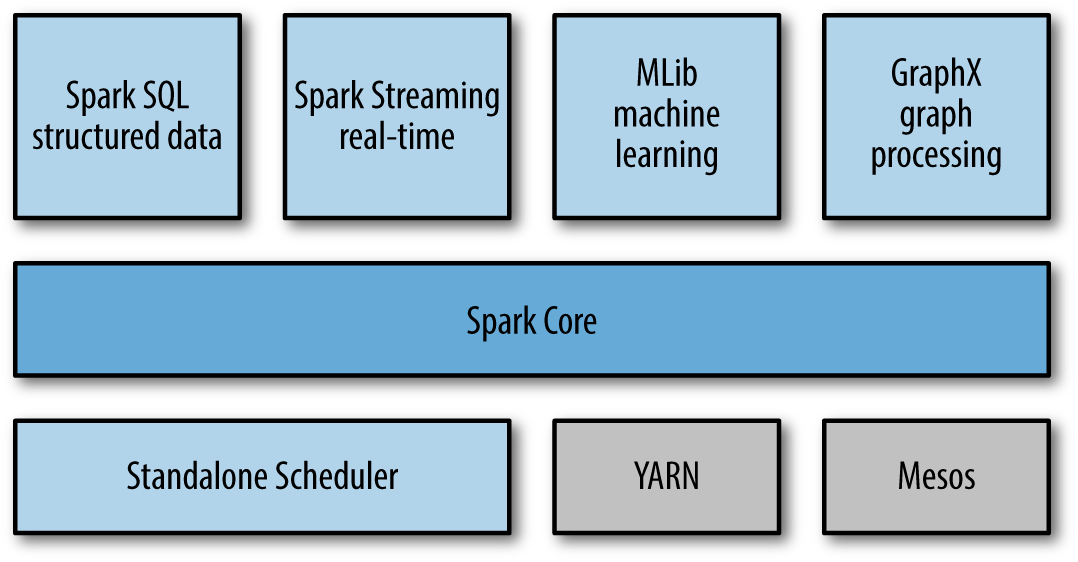
\includegraphics[width=14cm]{fig/lnsp_0101.png}
    \caption{Thành phần của Apache Spark\cite{orielly}}
    \label{fig:spark_compnent}
\end{figure}

\begin{itemize}
    \item Spark Core: \\
    Spark Core chứa các chức năng cơ bản của Spark, bao gồm các thành phần để lập lịch quản lý tác vụ, quản lý bộ nhớ, phục hồi lỗi hệ thông, tương tác với các hệ thống lưu trữ, v.v. Spark Core gồm những API xác định các bộ dữ liệu phân tán resilient distributed datasets (RDD) có khả năng phục hồi. RDD đại diện cho một tập hợp các thành phần phân tán được phân phối trên nhiều nút tính toán có thể được thao tác song song. Spark Core cung cấp nhiều API để xây dựng và thao tác với các thành phần đó.
    \item Spark SQL: \\
    Spark SQL là gói package khi làm việc với dữ liệu có cấu trúc. Nó cho phép truy vấn dữ liệu thông qua SQL cũng như Apache Hive và hỗ trợ rất nhiều nguồn dữ liệu bao gồm Hive tables, Parquest, JSON, ... Ngoài việc cung cấp giao diện SQL cho Spark, Spark SQL cho phép các nhà phát triển kết hợp các truy vấn SQL với các thao tác dữ liệu lập trình được hỗ trợ bởi RDD trong Python, Java và Scala, tất cả trong một ứng dụng, do đó có thể kết hợp SQL với các phân tích phức tạp.
    \begin{figure}
        \centering
        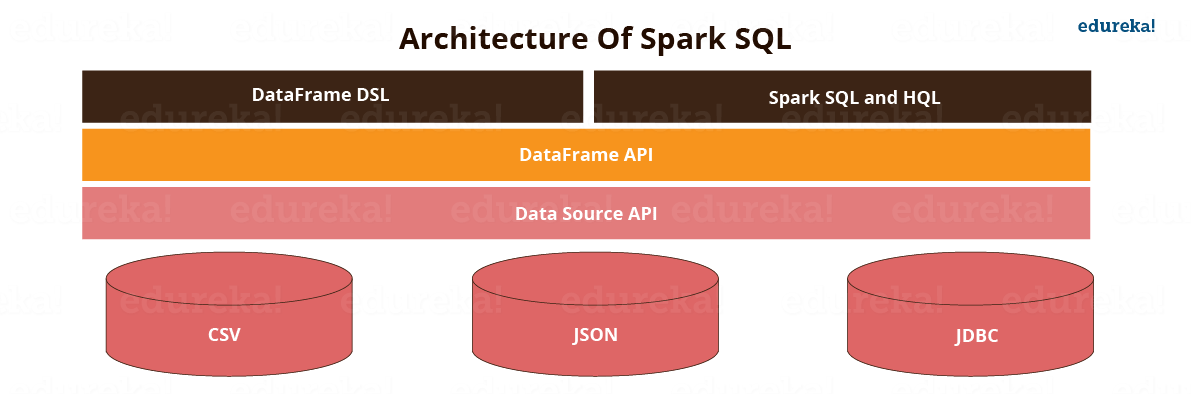
\includegraphics[width=16cm]{fig/spark_sql_component.png}
        \caption{Kiến trúc của SparkSQL\cite{spark_sql}}
        \label{fig:spark_architecture}
    \end{figure}
    \item Spark Streaming:\\
    Spark Streaming là một thành phần Spark cho phép xử lý các luồng dữ liệu cần xử lý trong thời gian thực. Ví dụ về các luồng dữ liệu bao gồm các logfiles được tạo bởi các máy chủ web tạo ra hoặc hàng đợi các tin nhắn có chứa các cập nhật trạng thái được tao bởi người dùng của một dịch vụ web. Spark Streaming cung cấp API để thao tác với các luồng dữ liệu khớp với API RDD của Spark Core, giúp các lập trình viên dễ dàng tìm hiểu dự án và di chuyển giữa các ứng dụng thao tác dữ liệu được lưu trữ trong bộ nhớ, trên đĩa hoặc đến thời gian thực. Bên dưới API của nó, Spark Streaming được thiết kế để cung cấp mức độ chịu lỗi, thông lượng cao và khả năng mở rộng tương tự như Spark Core.
    \item MLlib:\\
    MLib là một thành phần của Spark có thể giúp xử lý các tác vụ machine learning. Nó bao gồm các thuật toán học máy: phân loại (classification), hồi quy (regression), phân cụm (clustering), lọc cộng tác (collaborative filtering) cũng như hỗ trợ chức năng đánh giá mô hình dữ liệu và import dữ liệu để xử lý. 
    \item GraphX:\\
    GraphX là API của Spark cho đồ thị và tính toán trên đồ thị.
    \item Cluster Managers:\\
    Spark được thiết kế để có thể tăng hiệu năng tính toán bằng cách mở rộng hệ thống từ một đến hàng ngàn nút tính toán. Để đạt được khả năng như vậy trong khi vẫn tối đa tính linh hoạt, Spark dựa trên các công cụ quản lý cluster như Hadoop YARN, Apache Mesos hoặc công cụ quản lý cluster trong chính Spark là Standalone Scheduler. 
\end{itemize}
\newpage
\subsection{Docker\cite{DOCKER,docker}}
Docker là một công cụ dùng để đóng gói, vận chuyển và chạy container một cách đơn giản và dễ dàng trên các nền tảng khác nhau.\\
\\
Docker mang lại những giá trị cho người sử dụng:
\begin{itemize}
    \item Tính đóng gói (encapsulation): Không quan tâm đến việc thiếu các thư viện, thông tin cấu hình khi chạy ứng dụng. Có thể tạo một lần và chạy ở mọi nơi.
    \item Tính cô lập (isolation): tránh được xung đột khi chạy nhiều ứng dụng trên cùng một máy.
    \item Tính di động (portable): có thể dễ dàng chạy ứng dụng trên nhiều máy khác nhau. Không cần cài đặt lại.
    \item Có thể kịch bản hóa (script) hóa các công việc như kiểm thử tự động (automation testing), tích hợp (integration), đóng gói (packaging).
    \item Nhỏ gọn, chạy nhanh và ít tốn kém (overhead) hơn rất nhiều so với máy ảo (Virtual Machine).
\end{itemize}
\begin{figure}
    \centering
    
\includegraphics{fig/docker_facebook_share.png}
    \caption{Docker logo}
    \label{fig:docker_logo}
\end{figure}
\newpage
\subsubsection{Kiến trúc của Docker}
\begin{figure}
    \centering
    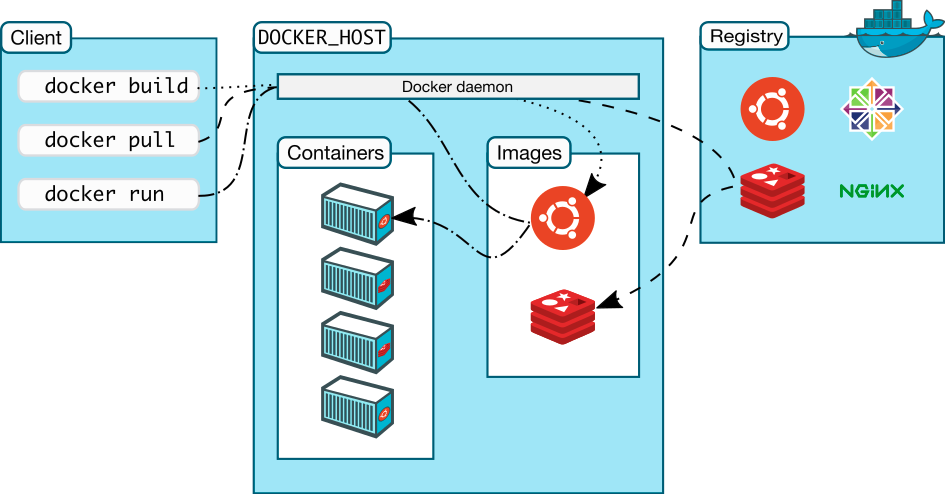
\includegraphics[width=16cm]{fig/docker_architecture.png}
    \caption{Kiến trúc Docker}
    \label{fig:docker_architecture}
\end{figure}
Docker là có kiến trúc Client-Server, gồm:
\begin{itemize}
    \item Docker Daemon: chạy ở trên host, đóng vai trò server, nhận các RESTful requests từ Docker Client và thực thi.
    \item Docker CLI: có vai trò là client, cung cấp giao diện tương tác với người dùng (command line) và gửi các RESTful requests tương ứng đến Docker Daemon.
    \item Docker Registry: private hay public registry, là nơi lưu trữ và chia sẻ các Docker Image.
\end{itemize}
\subsection{Một số khái niệm khác}
\begin{itemize}
    \item Docker Machine:tạo ra các Docker engine trên máy chủ.
    \item Docker Compose: chạy ứng dụng bằng cách định nghĩa cấu hình các Docker container thông qua tệp cấu hình.
    \item Docker image: một dạng tập hợp các tệp của ứng dụng, được tạo ra bởi Docker engine. Nội dung của các Docker image sẽ không bị thay đổi khi di chuyển. Docker image được dùng để chạy các Docker container.
    \item Docker Container: một dạng runtime của các Docker image, dùng để làm môi trường chạy ứng dụng.
\end{itemize}
\newpage
\subsubsection{Hoạt động của Docker}
\begin{figure}
    \centering
    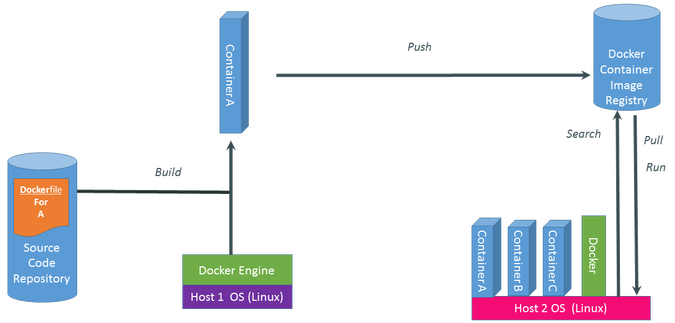
\includegraphics[width=16cm]{fig/basics-of-docker-system.png}
    \caption{Hoạt đông của Docker}
    \label{fig:process_docker}
\end{figure}
Như hình 7, ta thấy hoạt động của Docker được thực thi với 3 bước chính:\\
\\
\textbf{Build -> Push -> Pull,Run}\\
\begin{itemize}
    \item Build: Bước đầu tiên, tạo Dockerfile chứa các thông số cài đặt của ứng dụng. Dockerfile này được Build tại một máy tính đã cài đặt Docker Engine.\\
    Sau khi Build sẽ thu được Container chứa bộ thư viện và ứng dụng đã xây dựng.
    \item Push: Sau khi có được Container, chúng ta thực hiện push Container này lên đám mây và lưu trữ ở đó. Việc push này có thể thực hiện qua môi trường mạng Internet.
    \item Pull, Run: Giả sử một máy tính muốn sử dụng Container chúng ta đã push lên đám mây (máy đã cài Docker Engine) thì bắt buộc máy phải thực hiện việc Pull container này về máy. Sau đó thực hiện Run Container này.
\end{itemize}



%% --------- HIỆN THỰC ---------
\newpage
\section{HIỆN THỰC}
Trong giai đoạn đề cương, thực hiện các file như sau:
\begin{itemize}
    \item Ứng dụng: Chứa lệnh tạo Dockerfile và cài đặt các biến môi trường cần thiết tương ứng dành cho máy master và máy worker.
    \item Dockerfile: Là file được sinh ra từ ứng dụng. File Dockerfile được sinh ra chứa các câu lệnh cài đặt Java, Spark, Hadoop, Scala, Sbt, Python từ nền cơ bản là bản phân phối Ubuntu 16.04 LTS.
\end{itemize}
Phần mềm sẽ tạo nên các container tương ứng với các cài đặt cấu hình, tuy nhiên cần phải chỉnh sửa lại biến thông số về port tại hệ thống máy chủ chạy 2 container đó theo sự quản lý của người điều hành hệ thống SuperNode-XP.\\

Mô hình xử lý giai đoạn đề cương luận văn được mô tả theo sơ đồ sau:
\begin{figure}[h]
    \centering
    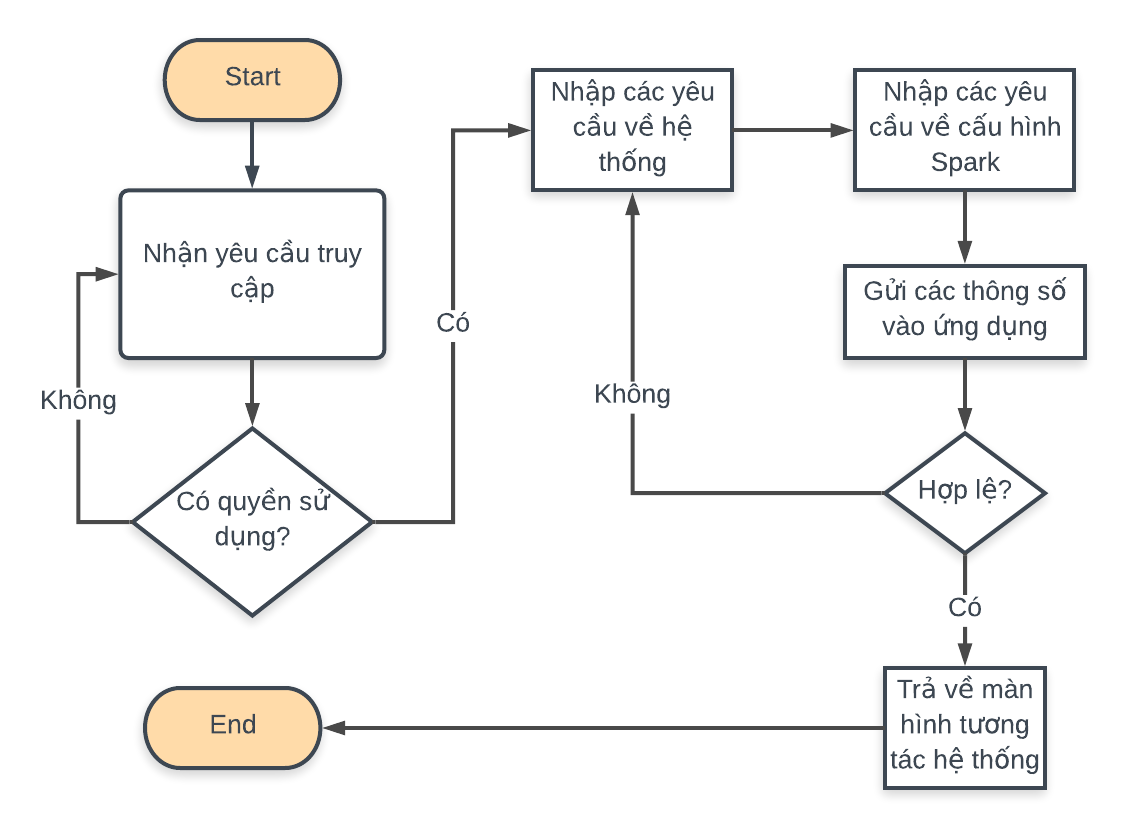
\includegraphics[width=16cm]{fig/diagram.png}
    \caption{Workflow giai đoạn đề cương LVTN}
    \label{fig:decuong_workflow}
\end{figure}
\newpage
\subsection{CÔNG CỤ ĐÁNH GIÁ HIỆU NĂNG}
Các công cụ đánh giá hiệu năng được lựa chọn:
\begin{itemize}
    \item Spark SQL Performance Tests của Databricks\cite{test_sql}: (Đánh giá hiệu năng của SparkSQL): Framework này hỗ trợ phiên bản Apache Spark 2.2 trở lên, thường xuyên được cập nhật. Bao gồm 11 điểm đánh giá được tổ chức thành 3 lớp nhắm vào các thành phần và chức năng khác khau của Spark:
    \begin{itemize}
        \item \textbf{DatasetPerformance: } So sánh hiệu suất của RDD API cũ với Dataframe mới và Dataset APIs.
        \item \textbf{JoinPerformance: } so sánh hiệu suất của join các bảng có kích thước và hình dạng khác nhau với kiểu join khác nhau.
        \item \textbf{AggregationPerformance: } so sánh hiệu suất tổng hợp các kích thước bảng khác nhau bằng các loại tổng hợp khác nhau.
    \end{itemize}
    \item Spark Performance Tests của Databricks\cite{test_spark}: Đánh giá hiệu năng của Spark, PySpark, Spark Streaming, và MLlib. Framework này hỗ trợ Apache Spark 1.0 trở lên. Rất đa dạng về mục đánh giá hiệu suất khi sử dụng các giải thuật machine learning: Generalized Linear Regression Model, Generalized Linear Classification Model, Alternating Least Squares, Matrix Multiplication, v.v
\end{itemize}
Cả 2 framework lựa chọn đều dễ sử dụng. Ngoài ra còn một số công cụ đánh giá khác: 
\begin{itemize}
    \item Spark DFSIO - Distributed IO benchmark tool\cite{spark_benchmarks}
    \item Spark-Bench\cite{spark_bench}
    \item BigDataBench
\end{itemize}


%% --------- TỔNG KẾT VÀ HƯỚNG PHÁT TRIỂN TRONG GIAI ĐOẠN LVTN ---------
\newpage
\section{TỔNG KẾT VÀ HƯỚNG PHÁT TRIỂN TRONG GIAI ĐOẠN LUẬN VĂN TỐT NGHIỆP}
\subsection{Mục tiêu đã hoàn tất trong giai đoạn đề cương luận văn}
Với những mục tiêu đã đề ra, nhóm đã thực hiện được các mục tiêu như sau:\\
\begin{itemize}
    \item Tìm hiểu hệ thống SuperNode-XP: Đã nắm được mục đích sử dụng, tiềm năng của hệ thống tính toán hiệu năng cao.
    \item Tìm hiểu công nghệ xử lý dữ liệu: Spark \& Hadoop: Nắm được tầm quan trọng, thành phần.
    \item Tìm hiểu về công nghệ container: Docker: Nắm được cấu trúc, cách thực hiện, của công nghệ container với đề tài.
    \item Các mô hình giải pháp đã có trên thế giới: Tìm được mô hình giải pháp mẫu.
    \item Các công cụ đánh giá hiệu năng hệ thống xử lý dữ liệu lớn: Tìm được một vài công cụ đánh giá hiệu năng, tuy nhiên chưa hoàn chỉnh, bước sang giai đoạn LVTN sẽ tiếp tục thử nghiệm thêm các công cụ đánh giá khác.
    \item Tạo các file script, Dockerfile chạy tự động các thiết lập cài đặt cấu hình: Đã viết được file cài đặt. Tuy nhiên chưa hoàn toàn tự động, sẽ tiếp tục cải tiến thêm trong giai đoạn LVTN.
    \item Chạy thử nghiệm trên hệ thống SuperNode-XP.
    \item Xác định hướng phát triển, xây dựng hệ thống trong giai đoạn Luận văn tốt nghiệp.
\end{itemize}
\\
Với yêu cầu đặt ra với hệ thống: Triển khai đơn giản, hiệu năng cao, bảo mật dữ liệu và thân thiện với người dùng, nhóm đặt ra mục tiêu và hướng phát triển trong giai đoạn LVTN như sau: \\
\begin{itemize}
    \item Tìm hiểu RDMA trên InfiniBand.
    \item Triển khai Hadoop \& Spark trên SuperNode-XP dùng Infiniband và đĩa cứng SSD.
    \item Tiếp tục tìm hiểu và thử nghiệm các công cụ đánh giá hiệu năng.
    \item Cải tiến ứng dụng sang hoàn toàn tự động.
    \item Thiết kế giao diện, tương tác với người sử dụng thân thiện: Người dùng có thể lựa chọn, nhập các yêu cầu về hệ thống, yêu cầu cài đặt Spark \& Hadoop.
    \item Các yêu cầu của người dùng có thể tự động tinh chỉnh theo hệ thống mà không cần can thiệp từ người quản trị hệ thống.
    \item Cải thiện hiệu năng của hệ thống.
\end{itemize}
\\
Sau khi kết thúc giai đoạn Luận văn tốt nghiệp, nhóm muốn hoạt động cấp phát của hệ thống sẽ hoàn toàn tự động và chỉ có người dùng tự tương tác với giao diện mà không cần phải cần sự can thiệp của người quản trị hệ thống theo như sơ đồ sau:\\
\begin{figure}
    \centering
    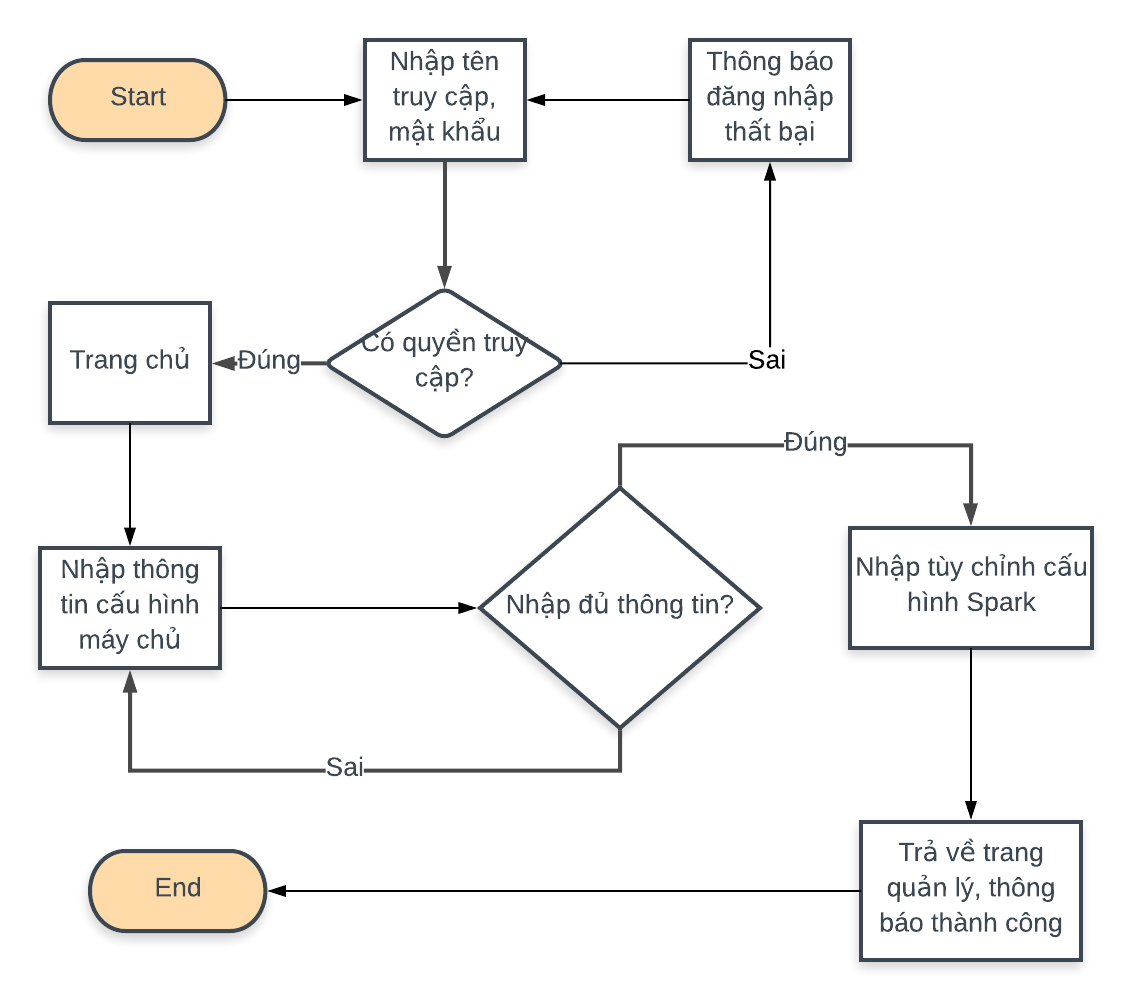
\includegraphics[width=16cm]{fig/luanvan_diagram.png}
    \caption{Workflow giai đoạn Luận văn tốt nghiệp }
    \label{fig:luanvan_diagram}
\end{figure}


%%%%%%%%%%%%%%%%%%%%%%%%%%%%%%%%% phụ lục
\newpage
\begin{thebibliography}{80}
\bibitem{SPARK_WIKI} 
Apache Spark (Wikipedia)
\\\texttt{https://en.wikipedia.org/wiki/Apache\_Spark}
\bibitem{HADOOP_WIKI} 
Apache Hadoop
\\\texttt{https://vi.wikipedia.org/wiki/Apache\_Hadoop}
\bibitem{DOCKER} 
Docker (Wikipedia)
\\\texttt{https://en.wikipedia.org/wiki/Docker\_(software)}
\bibitem{EC2} 
Amazon EC2 là gì?
\\\texttt{https://www.codehub.vn/Tim-Hieu-Ve-Amazon-EC2}
\bibitem{APACHE_WIKI} 
The Apache Software Foundation (Wikipedia)
\\\texttt{https://en.wikipedia.org/wiki/The\_Apache\_Software\_Foundation}
\bibitem{APACHE_HOME} 
The Apache Software Foundation Home
\\\texttt{https://www.apache.org/}
\bibitem{test_sql} 
Spark SQL Performance Tests
\\\texttt{https://github.com/databricks/spark-sql-perf}
\bibitem{test_spark} 
Spark Performance Tests
\\\texttt{https://github.com/databricks/spark-perf}
\bibitem{orielly} 
What Is Apache Spark? (Learning Spark - by Matei Zaharia, Patrick Wendell, Andy Konwinski, Holden Karau)
\\\texttt{https://www.oreilly.com/library/view/learning-spark/9781449359034/ch01.html}
\bibitem{spark_sql} 
Spark SQL Tutorial – Understanding Spark SQL With Examples
\\\texttt{https://www.edureka.co/blog/spark-sql-tutorial/}
\bibitem{docker} 
Docker
\\\texttt{https://devopsz.com/tag/docker/}
\bibitem{spark_benchmarks} 
Spark Benchmarks
\\\texttt{https://github.com/BBVA/spark-benchmarks}
\bibitem{spark_bench} 
Spark-Bench
\\\texttt{https://codait.github.io/spark-bench/}
\bibitem{BigDataBench} 
BigDataBench
\\\texttt{http://prof.ict.ac.cn/}
\bibitem{databrick} 
Databrick Cloud Community
\\\texttt{https://community.cloud.databricks.com/}


\end{thebibliography}
\end{document}
